
\section{OS - Intro}

\defn{Operating System}{a program which acts as an intermediary between the user and the hardware}

\par{The OS is the software which allows the user and higher level applications to communicate with the metal. It serves 3 main purposes:}

\begin{itemize}
	\item Usability
	\item Program Execution Scheduling and Control
	\item Efficiency Allocation of Resources
\end{itemize}

\subsection{Core Components}

	\defn{Kernel}{the program running at all times which is responsible for providing and API for the interaction between hardware and higher level programs; performing such tasks as reading and writing data to memory and determining how data received from and sent by \ita{I/O} devices is interpreted.}

	\defn{System Programs}{are programs which despite being associated with the OS do not form part of the kernel, they provide a platform for apps}

	\defn{Application Programs}{are programs which do not interact with the OS directly}

	\defn{BIOS}{the \ita{Basic Input Output System} is a special piece of software which comes preinstaled in the system's board ROM and is responsible for checking that the hardware is operation and loading the OS}

\subsection{Computer System Organization}

	\defn{Computer System}{can be defined as the interaction between four main components: \ita{Hardware, OS, Application Programs, Users}}

	\par{A modern computer system consists of 1+ CPUs and a number of device controllers which interact via a common bus that provides access between components and shared memory. It is the job of the device controller to transfer data between the devices and the local buffer storage which it maintains along with a set of special-purpose registers.}
	\par{The CPU and the device controllers can execute in parallel, competing for memory cycles. The three key aspects of the computer-system - Interrupts, Storage Structure, I/O Structure - are deigned in such a way so as to allow for memory to be used as efficiently as possible }

	\begin{figure}[H]
		\begin{center}
		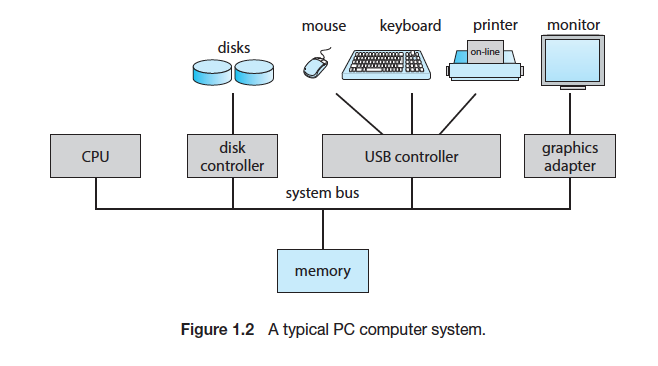
\includegraphics[width=\textwidth]{system}
		\end{center}
	\end{figure}


	\subsubsection{CPU Interrupts}

		\par{A typical operation of a program performing I/O:}

			\begin{enumerate}
				\item Device driver loads the registers in the controller
				\item Controller inspects data in order to know what action to execute
				\item Controller transfers data to local buffer
				\item Controller informs driver that operation has finished
				\item Driver gives back control to OS
			\end{enumerate}

		\par{The controller accomplishes 4 via an \ita{interrupt}. When hardware triggers an interrupt, the CPU stops the execution of all programs and it transfers execution to a fixed location which will usually contain the starting address for the interrupted service so that execution can restart when the interrupt routine finishes.}
		\par{Different architectures have different interrupt mechanisms, but they all share several essential functions, such as the transfer of control to the appropriate service routine. In order for this transfer to occur quickly a table of pointers to different interrupt routines - \ita{interrupt vector} - is kept in low memory and is used instead of an extra routine whose sole purpose would be to inspect the interrupt information. In this way the routine is called indirectly via the table.\mymarginpar{For implementation details see 1.2.1.2}}

		\begin{figure}[H]
		\begin{center}
		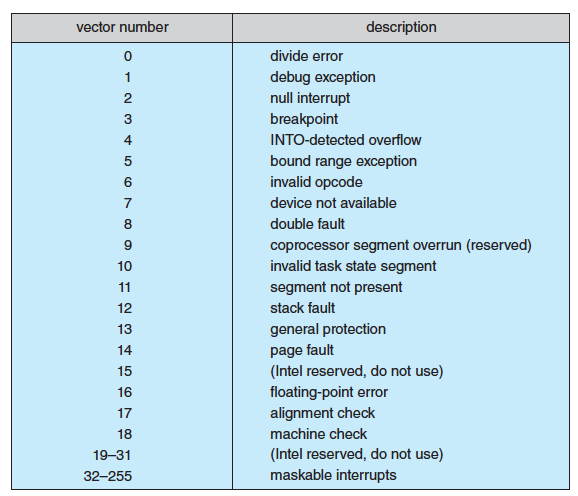
\includegraphics[width=\textwidth]{eventVector}
		\end{center}
	\end{figure}


	\subsection{Storage Structure}

	\par{When looking at a storage system one can pick out three main characteristics of importance, whose importance differs depending on their function and at which level of the system they are to be implemented, and which compete against each other. These are: \ita{Speed, Cost, Persistence/Volatility}}
	\par{Devices which need to process information immediately like the registers in the CPU are more costly,have a lower storage capacity and are in general volatile. In contrast, long-terms storage devices like the hard disk, or a flash drive are fairly inexpensive but their read/write speeds are significantly slower.}

	\begin{figure}[H]
		\begin{center}
		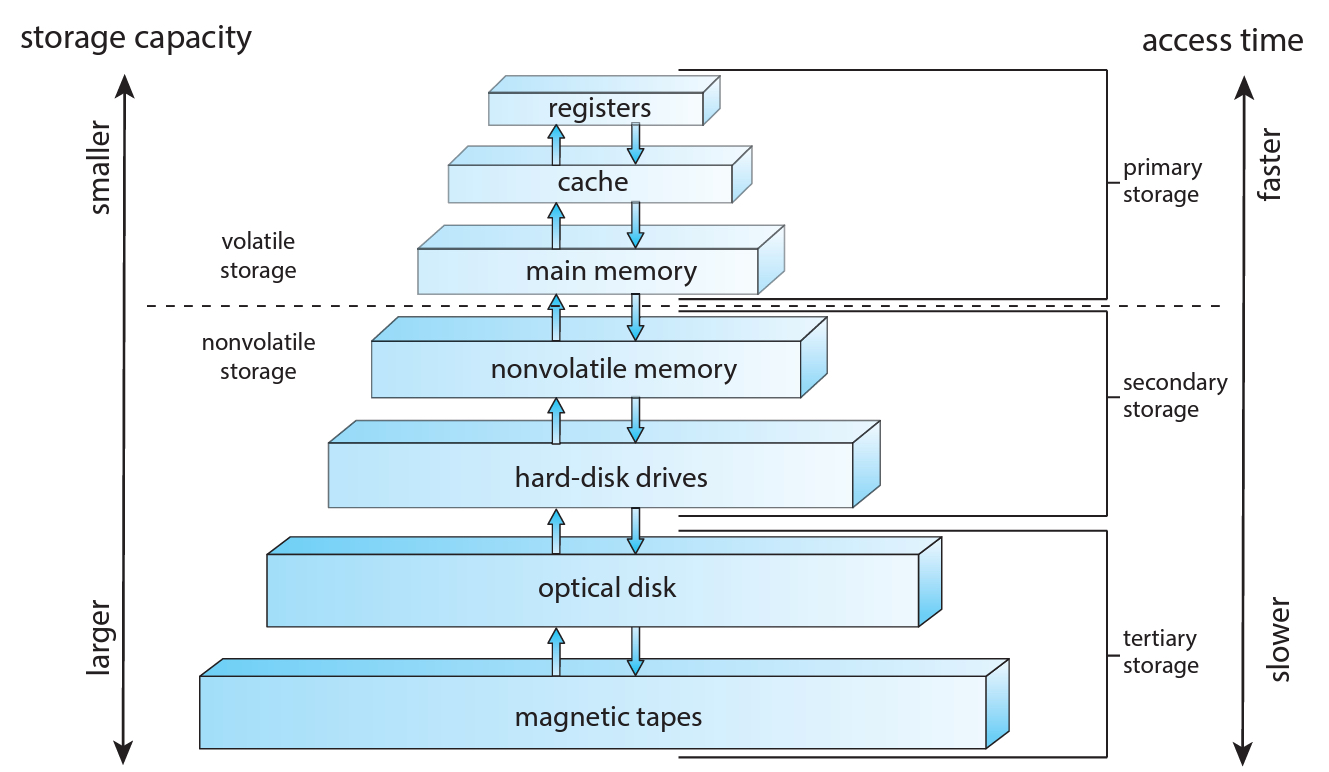
\includegraphics[width=\textwidth]{mem_hierarchy.jpg}
		\end{center}
	\end{figure}

	\defn{Caching}{the copy of information into faster storage systems}

	\subsection{I/O Structure}

	\par{A large chunk of OS code is dedicated to I/O management. Given the large amounts of data being moved by some I/O devices, the interrupt-driven cycle can produce high overhead instead direct memory access is used.}

	\defn{Direct Memory Access}{a resource-conserving and performance-improving operation for device controllers which allows devices to transfer large amounts of data directly to and from main memory, effectively bypassing the CPU and using instead a single purpose processor - \ita{DMAC}.}

\section{Computer-System Architecture}

	\par{The organization of a system can be categorized according to the number of general-purpose processors used.}

	\defn{Core}{the component that executes instructions and registers for storing data locally}

	\defn{CPU}{The hardware that executes instructions}

	\defn{Processor}{A physical chip that contains one or more CPUs}

	\subsubsection{Single-Processor}

	\par{The SP architecture uses a single CPU with a single processing core along with other device-specific processors which can only run a limited set of instructions.}

	\rem{This type of architecture is no longer present in modern computers}

	\subsection{Multiprocessor}

		\defn{Multicore}{a single CPU with more than one core who usually share some low-level memory}

		\defn{Throughput}{the amount of information which passes through the system}

		\par{Modern computers have 2+ processors each with a single core CPU. The processors share the computer bus, and may also share the clock, memory, and peripheral devices.The main advantage of this type of architecture is increased throughput, i.e. the higher number of processors allow for more data to be processed in less time}

		\rem{Increasing the number of processors by $N$ does not imply a $N$-fold increase in speed, since some of the processing power will be lost as overhead to tasks which make sure that the processors behave correctly when working together and sharing resources}

		\par{There are two main types of multiprocessor systems - \ita{Symmetric} and \ita{Asymmetric}, the former being the most common. They differ in the way tasks are split amongst different processors}

		\subsubsection{Symmetric}

			\par{In SMP each CPU processor performs all tasks, each CPU containing its own set of registers and private cache but all processors share access to the main memory. This has the advantage that many processes can run simultaneously\mymarginpar{$N$ processes can be running in a system with $N$ CPUs}. The downside of this type of system is that inefficiencies can occur by overloading one CPU while the other sits idle.}


		\subsubsection{Asymmetric}

			\par{Was the only way to handle multiprocessor systems before the invention of SMP. It is characterized by the fact that CPUs are not treated equally, i.e different CPUs prioritize certain tasks , like say I/O while others are reserved for system operations.}

	\subsection{Clustered}

		\par{The rationale behind clustered systems is similar to that of the multiprocessor systems, but we expand vertically, i.e instead of looking at multiple CPUs within a single computer, we use several computers within the same network.}
		\par{Clustered systems are very common nowadays and advancements in speed and computing power are linked to their pairing with SANs which are essentially local, dedicated data-storage networks. By having multiple machines connected to the same SAN if one machine goes offline another can quickly pick up the slack.}

		\defn{SAN}{describes a combination of hardware and software which essentially work together to form a dedicated storage area network}

		\defn{hot-standby mode}{one system runs parallel to another, in case the primary fails the backup quickly takes over}

		\defn{Asymmetric Clustering}{one machine in hot-standby mode}

		\defn{Symmetric Clustering}{multiple nodes running applications and monitoring each other}

\subsection{Process Management}

	\defn{Process}{a program in execution}

	\defn{Single-Thread}{single program counter which specifies the location of the next instruction to execute}

	\defn{Multi-Thread}{one program counter per thread}

	\par{In order to manage processes the system needs to be able to:}

		\begin{itemize}
			\item[]{Create and delete user and system processes}
			\item[]{Suspend and resume processes}
			\item[]{Provide mechanisms for process synchronization, communication and deadlock handling}
		\end{itemize}

\subsection{Memory Management}
	
	\par{Memory management is responsible for determining what is in memory, this includes:}

		\begin{itemize}
			\item[]{Tracking which parts of memory are in use and by whom}
			\item[]{Deciding which processes and data to move into and out of memory}
			\item[]{Allocate memory space as required}
		\end{itemize}

\subsection{Storage Management}

	\par{Storage management concerns itself with the management of the file-system, in particular how the OS handles free space and how that free space is split into files and directories with appropriate access permissions so that the user can easily access them.}



